\chapter{Das Actor-Model} \label{actor:chapter}
Das von \cite{hewitt1973session} erstmals vorgestellte theoretische Software Model, ermöglicht das Entwerfen und Erstellen von parallelisierten Softwaresystemen. Es unterstützt Softwareentwickler bei der effizienten Nutzung von Mehrkernprozessoren sowie bei Handhabung der  Komplexität mit welcher die Nebenläufige Programmierung einhergeht.   
% evt. ausbau um probleme mit nebeläufiger programmierung
\\
Neben geläufigen Modellen wie beispielsweise die Funktionale Programmierung oder die Objektorientierte Programmierung, bietet das Actor-Model eine Vorgehensweise Software zu schreiben. Dieses Kapitel wird die theoretischen Grundlagen des Actor-Models aufzeigen und sich in drei Teile unterteilen. Zuerst wird das Actor-Model in seiner Grundform wie von \cite{hewitt1973session} und \cite{Agha1985ActorsSystems} definiert gezeigt, anschließend werden Architekturkonzepte auf Basis des Actor-Model erarbeitet und abschließend erfolgt eine Evaluierung des Actor-Models.

\section{Reactive Manifesto}
\label{reactiveManifesto}
Das \textit{Reactive Manifesto} (siehe \cite{reactiveManifesto}) ist eine Sammlung an grundlegenden Anforderungen, welche eine verteilte Softwarearchitektur erfüllen soll, um die Verarbeitung großer Datenmengen in der Größenordnung von bis zu mehreren Petabytes in der Millisekunden bewerkstelligen zu können. 
\graffito{Ein Petabyte sind $10^{15}$ \textit{Bytes}, oder $1000$ \textit{Terabytes}}
Wie in \cite{reactiveManifesto} angegeben, ist das \textit{Reactive Manifesto} bestens geeignet um Cloud-Anwendungen zu erstellen, welche in mehreren Rechenzentren verteilt betrieben werden. \\
Die Autoren des Manifestes fordern von einer Anwendung vier grundlegende Eigenschaften damit sie dem \textit{Reactive Manifesto} entsprechen und somit als reaktive Anwendung angesehen werden kann. Das Manifest sieht folgende Anforderungen als Grundstein für eine erfolgreiche Softwarearchitektur, welche für verteilte Applikationen entworfen wird. 
\begin{description}
  \item[Antwortbereit]\label{reactivo:responsive}
  Ein reaktives System antwortet auf alle Anfragen immer innerhalb eines vorab definierten Zeitfensters. Der einzige Umstand der zu keiner Antwort führt, ist jener, wenn das System in einem Fehlerzustand ist. In allen anderen Fällen muss auf jede Anfrage innerhalb des Zeitfensters eine Antwort gesendet werden.
  Laut \cite{reactiveManifesto} ist diese Regel der Grundstein einer reactiven Applikation.
  \item[Widerstandsfähig]\label{reactivo:resilient}
  Bei einem Ausfall von Komponenten des Systems, wie Hard- oder Software, wird die Anforderung \textit{Antwortbereitschaft} des Systems nicht beeinflusst. Daher darf ein Ausfall einer Komponente keine Auswirkungen auf das Antwortverhalten der Applikation haben.\\
  Widerstandfähigkeit kann laut \cite{reactiveManifesto} durch Delegieren von Verantwortung an verschiedene Komponenten sowie das Replizieren von Komponenten erreicht werden. Weiters ist durch Isolation der Komponenten zu verhindern, dass ein Fehler einer Komponente auf andere Komponenten übergreift. Dadurch bleibt der Ausfall einer Komponente für das gesamte System ein überschaubares Problem. Ebenfalls ist es notwendig, beim Auftritt eines Fehlers im System die Behebung so schnell wie möglich durchzuführen, im Idealfall erfolgt dies automatisch.
  \item[Elastisch]\label{reactivo:elastic}
  Das Antwortverhalten einer Reactiven Anwendung darf durch einen plötzlichen Anstieg der eintreffenden Anfragen und der damit erhöhten Last nicht beeinträchtigt werden. Dies kann erreicht werden, indem, ähnlich wie bei der Wiederstandfähigkeit, auf Replizierung der Komponenten gesetzt wird. Jedoch wird für die Elastizität des System auf eine automatische Replikation der betroffenen Komponenten gesetzt. Vor dem Erreichen der Maximallast einer Komponente wird diese an einem anderen Ort repliziert und teilt sich somit die Last. 
  \item[Nachrichtenorientiert]\label{reactivo:messageDriven}
  Ein reactives System besteht, wie aus den vorhergegangenen Anforderung abzuleiten ist, aus mehreren gelösten Komponenten. Die Kommunikation zwischen den Komponenten muss, um als Reactive zu gelten, laut \cite{reactiveManifesto} über asynchrone Nachrichten erfolgen. Durch den Einsatz von Asynchronität ist eine Komponente während der Kommunikation mit einer anderen Komponente nicht von dieser abhängig. Weiters können Nachrichten ortsungebunden versendet werden. Dies ermöglicht somit die Skalierung von Komponenten. 
\end{description} 
Die vier Anforderungen Antwortbereitschaft, Widerstandfähigkeit, Elastizität und Nachrichtenorientiertheit müssen in einer Applikation zu jedem Zeitpunkt gewährleistet werden und in der Konzeptionsphase einer reaktiven Anwendung immer mit einfließen. Durch die Einhaltung dieser vier Grundrichtlinien kann eine Anwendung von vornherein auf Verteilung und Skalierung entworfen werden.\\

Die Anforderungen des \textit{Reactive Manifesto} ähneln der Definition des Actor-Models (siehe Abschnitt \ref{actor:definition}). Laut \cite{Vernon2015ReactiveAkka} ist das Actor-Model die führende Architektur bei der Implementierung und Umsetzung von reaktiven Anwendungen, jedoch schließt das reaktive Manifest andere Softwaremuster nicht aus. \\
Bei der Umsetzung einer Softwarearchitektur mit dem Actor-Model, sind die Anforderungen Elastizität sowie Nachrichtenorientiertheit des \textit{Reactive Manifesto} implizit gegeben, da das Actor-Model diese, wie in den Kapiteln \ref{actor:definition} und  \ref{actor:Mailbox} beschrieben, explizit vorgibt.\\
Eine Applikation, welche korrekt mit dem Actor-Model umgesetzt wird, kann als Reactive Applikation angesehen werden wenn die Anforderung \textit{Widerstandfähigkeit} miteingebracht wird. Diese ist im Actor-Model nicht definiert, jedoch bieten moderne Implementierungen des Actor-Models diese Anforderung im Form von \textit{Supervision}, siehe hierzu Abschnitt \ref{actor:supervision}.


\section{Actor-Model Definition}\label{actor:definition}
In der ersten Definition des Actor-Models von \citep{hewitt1973session} wird ein Actor beschrieben, als kleinster Bestandteil einer Software. Jeder Bestandteil eines Software Skriptes, welches benötigt wird um einen Programmablauf zu ermögliche, ist demnach als Actor zu betrachten. Hierzu zählen Datenstrukturen, auch primitive Datentypen, logische Verknüpfungen und auch Benutzereingaben oder Berechnungsergebnisse. All diese Bestandteile haben ein bestimmtes Verhalten und reagieren unterschiedlich auf äußere Einwirkungen. Alle Bestandsteile des Codes interagieren untereinander, in dem sie sich gegenseitig Nachrichten senden und auf diese entsprechend reagieren.\\
Das Actor-Modell kann als mathematisches Modell für parallele Datenverarbeitung, welches Akteure als universelle Grundlage der parallelen Verarbeitung verwendet, gesehen werden. Im Gegensatz zu anderen Modellen wurde das Actor-Modell von der Physik unserer Umwelt inspiriert. \footnote{Auch in der realen Welt werden Informationen nur über Nachrichten untereinander ausgetauscht. Jede Interaktion zur Umwelt erfolgt, in dem man einen Impuls an ein anderes Objekt gibt. Wenn wir beispielsweise den Namen einer Personen wissen wollen, können wir diesen nicht einfach ablesen, vielmehr müssen wir die Person nach deren Namen fragen. Ist die Person gewillt dem Fragenden diese Auskunft zu erteilen, antwortet sie mit einer anderen Antwortnachricht darauf. In welcher Form diese Nachrichten übermittelt werden (Sprache, Brief, Gesten etc. ), ist nicht relevant.} \citep{Vernon2015ReactiveAkka} .  In modernen Implementierungen des Actor-Models, ist jedoch ein Actor nicht der kleinste Bestandteil eines Skriptes, hier wird vielmehr versucht, wie unter \ref{?}  beschrieben, die kleinst mögliche Aufgabe einer Software als Actor abzubilden. \\
Weiters kapseln Actoren zusammengehörende Informationen und beinhalten auch ein Verhalten dieser.  Grundsätzlich lässt sich sagen, dass die Interaktion durch Nachrichten mit anderen Actors sowie das Kapseln des eigenen Verhalten einen Actor auszeichnet.

\subsection{Actor}
Ein Actor ist eine logische, atomare Einheit welche Nachrichten empfangen kann. Nachrichten sind die einzige Möglichkeit wie Actors untereinander, sowie mit externen Komponenten, kommunizieren können \citep{Agha1985ConcurrentParallelism}. Nachrichten werden an einen Actor gesendet und von diesem abgearbeitet. Dabei muss ein Actor folgende Bedingungen erfüllen.

\begin{description}
    \item[1. Kein Zugriff von außen]\label{actor:requirements:shareNothing}
    Die interne Repräsentation eines Actors ist nur für den Actor selbst bestimmt. Es darf keine Möglichkeit geben Werte eines Actors von anderen Actoren oder sonstigen Codestellen zu lesen oder zu manipulieren. Änderungen und lesezugriffe sind ausschließlich über Nachrichten möglich (siehe \ref{actors:messages}). 
    \item[2. Asynchrone Kommunikation]\label{actor:requirements:AsynchronCommunication}
    Kommunikation mit anderen Actoren erfolgt Asynchrone. Wird eine Nachricht an einen anderen Actor gesendet, wird nicht auf eine Antwort von diesem gewartet. Somit ist eine zügige Abarbeitung einer Nachricht möglich.
    \item[3. Sequentielle Abarbeitung von Nachrichten]
    Jeder Actor kann gleichzeitig exakt eine Nachricht zu gleichen Zeit abarbeiten. Alle anderen Nachrichten müssen in einer Warteschlange auf die Abarbeitung warten (siehe \ref{actor:Mailbox}).
    \item[4. Frei von Sperrmechanismen]
    Durch die Bedingungen {1.} und  {3.} ist es ausgeschlossen, dass ein Codeteil innerhalb eines Actors von außen, oder gar von einem anderen Thread, ausgeführt wird. Daher sind Sperrmechanismen, wie unter \ref{actor:parallelism} beschrieben, nicht nötig.
    \item[5. Kleinst mögliches Aufgabengebiet]
    Ein einzelner Actor soll ein möglichst kleines Aufgabengebiet behandeln und andere Aufgaben an andere Actoren abgeben. Dadurch wird einerseits ein hoher Durchsatz gewährleistet und einerseits die Komplexität eines einzelnen Actors vermindert.
\end{description}

\subsubsection{Arbeitsaufgaben und Nachrichten}\label{actors:messages}
In \cite{Agha1985ActorsSystems} wird beschrieben, dass in einem Actor-System eine beliebige Anzahl an zu bearbeitendenden Arbeitsaufträgen vorliegt. Diese Aufgaben werden in einem Actor-System zwischen den Actors zugewissen. Während der Abarbeitung einer Aufgabe können neue Aufgaben erstellt und in das Actor-System eingebracht werden. Eine Aufgabe wird im Kontext eines Actor-Systems wie folgt repräsentiert:
\begin{description}
    \item[Identifikation] Jede Aufgabe bekommt eine eindeutige Identifikation, welche sie von anderen Aufgaben unterscheidbar macht.
    \item[Ziel Adresse] Adresse an wenn der Auftrag gerichtet ist.
    \item[Aufgaben Inhalt] Beinhaltet alle benötigten Informationen um diese Aufgabe abzuarbeiten
\end{description} 
Um eine neue Aufgabe zu erstellen muss somit die Adresse bekannt sein an welche diese gerichtet wird. Hier wird von \cite{Agha1985ActorsSystems} drei mögliche Wege aufzeigt wie ein Actor eine solche Adresse während der Abarbeitung einer anderen Aufgabe erhalten kann.
\begin{description}
    \item[Bereits bekannt] Die Adresse eines anderen Actors ist durch die bearbeitung früherer Aufgaben bereits bekannt.
    \item[In Ihnalt enthalten] Im Inhalt der gerade bearbeitenden Aufgabe ist eine andere Adresse enthalten.
    \item[Neuer Actor] Während der abarbeitung der aktuellen Aufgabe wird ein neuer Actor erstellt. Durch das erstellen des Actors ist auch dessen Adresse bekannt.
\end{description}
In aktuellen Interpreterionen eines Actors, wie beispielsweise \cite{Vernon2015ReactiveAkka} oder \cite{Brown2016ReactiveAkka.net.} wird jedoch nicht mehr von Aufgaben sondern nurmehr von Nachrichten gesprochen. Diese enthalten jedoch ebenfalls immer eine Adresse sowie einen Nachrichteninhalt. Die Identifikation der Nachricht wird in modernen Systemen jedoch nicht mehr verwendet. \\
\subsubsection{Actor Verhalten}
\label{actorBehaviour}
Empfängt ein Actor eine Nachricht welche für ihn bestimmt ist, so kann dieser auf mehrere unterschiedliche Arten reagieren. In \citep{Agha1985ActorsSystems} und \citep{Vernon2015ReactiveAkka} werden folgende möglichkeiten eines Actors beschrieben:
\begin{description}
    \item[Neue Nachricht erstellen] Erfordert die bearbeitung der empfangen Nachricht neue Berechnungen, kann eine, oder auch mehrere neue Nachrichten erstellt werden. Diese Nachrichten können dann an andere Actors, gesendet werden. Auch Resultate welche durch die bearbeitung der Nachricht erfolgen können so bekannt gegeben werden.
    \item[Actor erstellen] Sind teile der aktuellen Nachricht nicht vom bearbeitenden Actor bearbeitbar, kann von diesem ein neuer Actor erstellt werden welcher für diese Aufgabe besser geignet ist. Diesem neuen Actor wird dann eine Nachricht mit der Teilaufgabe zugesendet.
    \item[Verhalten ändern] Das Resultat einer bearbeitung kann sein, dass die Verarbeitung der nächsten Nachrichten an diesen Actor in einer anderen Art und Weiße erfolgen muss. Daher kann der Actor sich für die nächste Nachricht ein neues verhalten bestimmen.
    \item[Zustand verändern] Während der abarbeitung einer Nachricht kann der Actor auch seinen eigenen privaten Zustand verändern.
\end{description}
% Das erstellen von neuen Actors während der Behandlung einer empfangen Nachricht ermöglicht es, komplexe oder Zeitintensive Rechenaufgaben auf andere Actors auszulagern. Da die Abhandlung einer Nachricht, wie bereits erwähnt, pro Actor sequentiell erfolgt und innerhalb eines Actors keine direkte parallelität erlaubt ist

\subsubsection{Nachrichten Eingang}\label{actor:Mailbox}
Jeder Actor kann jederzeit an jeden anderen Actor in einem System eine Nachricht zukommen lassen. Da ein einzelner Actor jedoch zur gleichen Zeit nur exakt eine Nachrichten bearbeitend kann muss gew sein das wartende Nachrichten nicht verloren gehen. Nachrichten an ein Actor werden nach dem {FIFO-Prinzip} abgearbeitet. 
\graffito{Bei {First In, First Out}, kurz {FIFO}, wird immer die älteste Nachricht in einer Warteschlange behandelt.} Um dies zu gewährleisten, benötigt ein Actor eine Nachrichten Warteschlange.\citep{Agha1985ActorsSystems}. Eine abgeschlossene Nachricht kann abschließend verworfen werden. 

\subsubsection{Parallelität}\label{actor:parallelism}
Obwohl ein Actor ankommende Nachrichten nur sequentiell bearbeitend kann, ist das Actor-Model Ideal für parallele Aufgaben.\citep{hewitt1973session} Durch das weiterreichen von Subaktionen an andere Actoren ist jedoch höchste Parallelität gegeben. In einem laufenden Actor-System sind meist eine vielzahl an einzelnen Actors parallel am Nachrichten abarbeiten. Dadurch kann ein Mehrkernprozessor optimal genützt werden. \citep{Agha1985ActorsSystems} \\
Durch die gleichzeitige Bearbeitung von maximal einer Nachricht pro Actor sowie die Unterbindung von Lesezugriffen auf den eigenen, internen State durch andere Actors (siehe \ref{actor:requirements:shareNothing}), benötigt es keine Sperrmechanismen innerhalb eines Actors. Dadurch wird erstens der Sourcecode übersichtlicher und zweitens entfällt das aufwändige allokieren von Sperreressourcen.\citep{Vernon2015ReactiveAkka}
Wird nun bedacht das ein Actor grundsätzlich nur jeweils für eine kleine Aufgabe optimiert wird, und andere Aufgaben an andere Actors abgibt, wird mit dem entfallen von Sperrmechanismen die Abarbeitungszeit für eine einzelne Nachricht pro Actor auf ein absolutes minimum gebracht. \citep{Vernon2015ReactiveAkka} \\
Zu beachten ist bei diesem Konzept das bei der Abarbeitung einer Nachricht nicht auf eine andere Nachricht gewartet werden soll. Dies führt zu neuen Architekturmustern welche Auszugsweise unter \ref{theory:actorArchitecture} beschrieben werden.

\subsection{Actor-System}
Ein einzelner Actor alleine kann Aufgrund seiner begrenzten möglichkeiten nur relativ wenig bewirken. Der große Vorteil erwirkt das Actor-Model erst durch die Macht von vielen einzelnen Actors welche miteinander interagieren. Eine solche Bildung von vielen Actors wird als Actor-System bezeichnet.\citep{Agha1985ActorsSystems}
\subsubsection{Kommunikation ausserhalb des Systems}
Nachrichten werden prinzipiell nur unter Actors innerhalb eines Actor-System ausgetauscht. In \cite{Agha1985ActorsSystems} wird erläutert, dass für die kommunikation mit Komponenten außerhalb eines Actor-System sogenannte Rezeptionisten Actors benötigt werden.\\
Ein solcher Rezeptionist ist prinzipiell ein gewöhnlicher Actor, welcher jedoch darauf Spezialisiert ist mit nicht Actors zu kommunizieren. Dafür benötigt ein solcher Rezeptionist eine definierte Schnittstelle. Über diese Schnittstelle können dann Codeteile (Webservices, GUI Implementieren usw..) Nachrichten in ein Actor-System einbringen. Weiters ist es auch über diese speziellen Actors möglich auf eine Antwort einer eingebrachten Nachricht zu warten. Die eigentliche Abarbeitung der externen Nachricht wird vom Rezeptionist an dafür zuständige Actors innerhalb des Actor-Systems geliefert.\citep{Agha1985ActorsSystems}\\
Neben der Möglichkeit vom Einsatz eines Rezeptionisten um mit externen Komponenten zu kommunizieren wird in \cite{Agha1985ActorsSystems} auch die Möglichkeit beschrieben mit externen Actor-System zu interagieren. Dies ist Nötig um beispielsweise zwei getrennt Entwickelte Actor-Systeme zu verbinden. Hierfür wird ein Set an externen Actoren definiert. Diese wissen zwar von der existenz eines externen Actor-Systems, kennen aber dessen Implementierung nicht. Über definierte externe Actoren können so trotzdem Nachrichten zwischen zwei fremden Actor-Systemen ausgetauscht werden. \\
Ohne den Einsatz von zumindest eines Rezeptionist oder eines externen Actors kann ein Actor-System nicht mit der Umwelt interagieren, da es der einzige Weg ist Nachrichten und somit Informationen von außen zu empfangen und ebenso Ergebnisse nach außen zu geben. 

\section{Actor Grafik Legende}\label{actor:diagram:description}
Um den Ablauf in einem Actor-System besser zu verstehen bittet sich die visuelle Darstellung in Form von Diagrammen eines Actors oder eines Actor-Systems an. In den Werken \cite{kuhn2017reactive} und \cite{Vernon2015ReactiveAkka} wurde eine einheitliche, grafische Notation für das Actor Model vorgeschlagen, welche auch für diese Arbeit herangezogen wird. Im folgenden nun eine kleine Einführung in diese Notation, welche die für diese Arbeit notwendigen Notationen darstellt und deshalb kein Anspruch auf Vollständigkeit stellt.\\
\subsection{Actors darstellen}
    Ein einzelner Actor wird als Kreis dargestellt, innerhalb dieses Kreises steht der Name des Actors. In Abbildung~\ref{fig:actor:diagram:longLiveActor} wird ein Actor dargestellt welcher persistent existiert, im gegensatz dazu steht ein Actor welcher nur für eine kurze Zeit existiert dieser wird mit gestrichelter Linien, siehe Abbildung~\ref{fig:actor:diagram:shortLiveActor}, dargestellt. Ein Actor welcher nur für kurze Zeit existiert, wird meist verwendet um eine einzelne spezielle Nachricht abzuarbeiten.
\begin{figure}
    \centering
    \begin{minipage}{.5\textwidth}
      \centering
      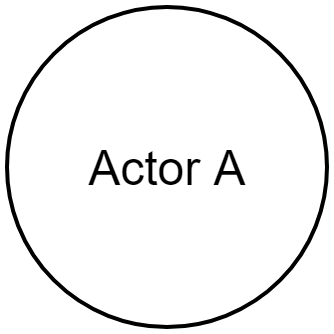
\includegraphics[width=.5\linewidth]{gfx/actor/longLiveActor}
      \captionof{figure}{Ein einfacher Actor.}
      \label{fig:test1}
    \end{minipage}%
    \begin{minipage}{.5\textwidth}
      \centering
      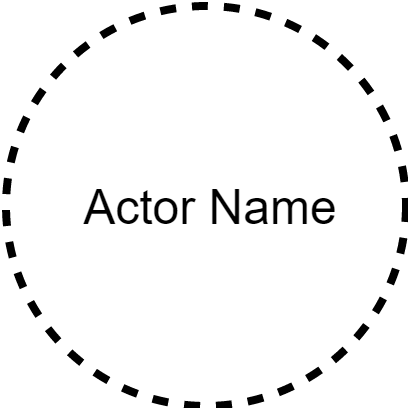
\includegraphics[width=.5\linewidth]{gfx/actor/shortLiveActor}
      \captionof{figure}{Ein Actor welcher direkt nach der Abarbeitung einer Nachricht wieder zerstört wird.}
      \label{fig:test2}
    \end{minipage}
    \end{figure}  

\subsection{Nachrichten erstellen}
Das erstellen einer Nachricht durch den Actor {A} sowie die Zustellung durch den Actor {A} and den Actor {B} wird in Abbildung~\ref{fig:actor:diagram:simpleCreateAndSendMessage} abgebildet. Wichtig ist hier, dass der Actor {A} nicht nur die Nachricht sendet, sondern sie auch erstellt!
\begin{figure}
    \centering
    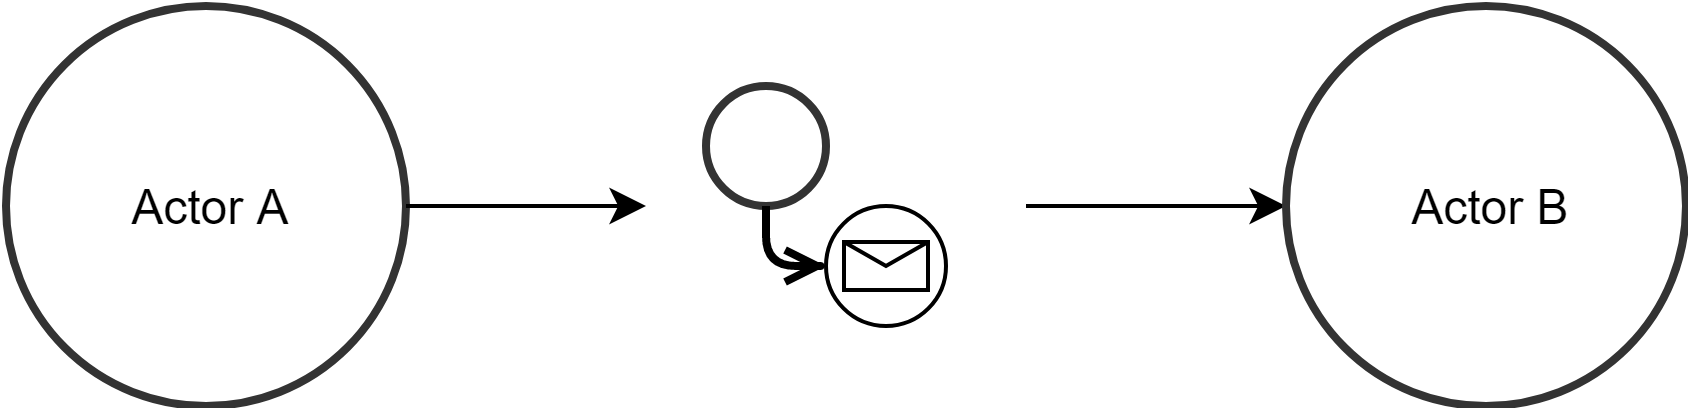
\includegraphics[width=\linewidth]{gfx/actor/simpleCreateAndSendMessage}
    \caption{Actor {A} erstellt eine neue Nachricht und sendet sie an Actor {B}.}
    \label{fig:actor:diagram:simpleCreateAndSendMessage}
\end{figure}

\subsection{Actors erstellen}
Das erstellen von Actoren durch einen Actor wird durch zwei kreise abgebildet. In Abbildung~\ref{fig:actor:diagram:childActorCreation} erstellt der {Parent}-Actor einen neuen Actor, den sogenannten {Child}-Actor.
\begin{figure}
    \centering
    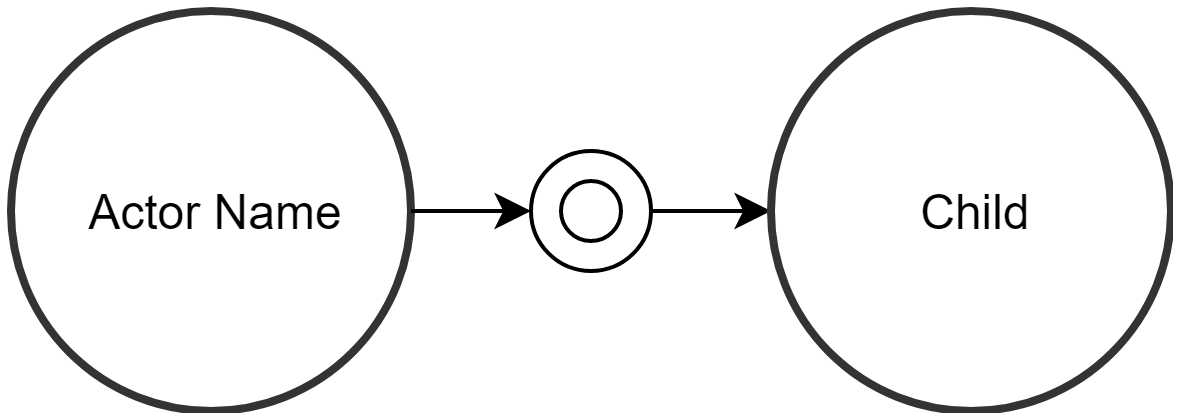
\includegraphics[width=\linewidth]{gfx/actor/childActorCreation}
    \caption{Ein Actor erstellt einen neuen Actor}
    \label{fig:actor:diagram:childActorCreation}
\end{figure}

\subsection{Darstellung eines Ablaufes}
Um einen konkreten Ablauf eines Actors darstellen zu können, benötigt man die darstellung der Nachrichteneingangsreihenfolge. Diese wird von \cite{kuhn2017reactive} und \cite{Vernon2015ReactiveAkka} als Linie dargestellt auf welcher sich Kreise befinden. Die abarbeitung wird von oben nach unten dargestellt. In Abbildung~\ref{fig:actor:diagram:asynchronMessageReceivment} bekommt der Actor zwei Nachrichten zugesendet, und sendet eine Nachricht dazwischen ab. Durch diese Abbildung ist es möglich, sequentielle Abläufe darzustellen
\begin{figure}
    \centering
    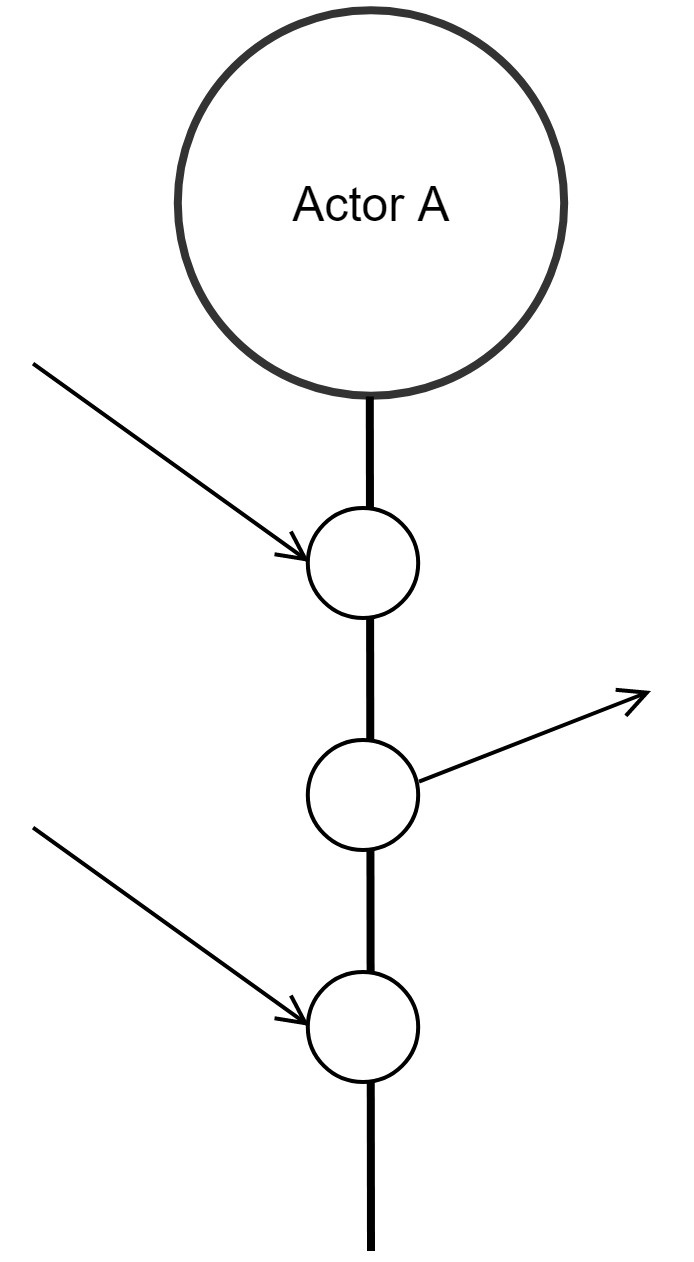
\includegraphics[height=6cm]{gfx/actor/actorAsynchMessgeFlow}
    \caption{Asynchroner Ablauf eines Actors.}
    \label{fig:actor:diagram:asynchronMessageReceivment}
\end{figure}

\section{Noch einzuordnern}
\subsection{Supervision}\label{actor:supervision}
\subsection{Location Transparent}{actor:locationTransparency}
\section{Actor basierte Architekturmuster}
\label{theory:actorArchitecture}
\section{Evaluierung}
%todo
%Agha zitate kontrollieren